\documentclass{report}
\usepackage[utf8]{inputenc}
\usepackage[francais]{babel}
\usepackage[T1]{fontenc}
\usepackage{lmodern}
\usepackage{textcomp}
\usepackage{listings}
\usepackage{graphicx}
\usepackage{hyperref}
\usepackage{titlesec}
\usepackage{tcolorbox}
\usepackage{amsmath}
\usepackage{color}
\usepackage{multirow}
\setcounter{tocdepth}{5}
\setcounter{secnumdepth}{4}
\definecolor{dkgreen}{rgb}{0,0.6,0}
\definecolor{gray}{rgb}{0.5,0.5,0.5}
\definecolor{mauve}{rgb}{0.58,0,0.82}
\definecolor{gray}{rgb}{0.4,0.4,0.4}
\definecolor{darkblue}{rgb}{0.0,0.0,0.6}
\titleformat{\paragraph}
{\normalfont\normalsize\bfseries}{\theparagraph}{1em}{}
\titlespacing*{\paragraph}
{0pt}{3.25ex plus 1ex minus .2ex}{1.5ex plus .2ex}
\renewcommand{\thesection}{\Roman{section}}
\hypersetup{
    colorlinks=true,
    linkcolor=black,
    filecolor=magenta,
    urlcolor=cyan,
}
\lstnewenvironment{cc}
{
\lstset{frame=tblr,
  language=C,
  aboveskip=3mm,
  belowskip=3mm,
  showstringspaces=false,
  columns=flexible,
  basicstyle={\small\ttfamily},
  numbers=none,
  numberstyle=\tiny\color{gray},
  keywordstyle=\color{blue},
  commentstyle=\color{dkgreen},
  stringstyle=\color{mauve},
  breaklines=true,
  breakatwhitespace=true,
  tabsize=3
}}
{}

\begin{document}
\title{
  \begin{minipage}\linewidth
      \centering
      
\includegraphics[width=40mm]{resources/01.png}\vskip 20pt
      Rapport TP4 : Configuration complète d'un serveur
      \vskip 5pt
      \author{
        DRISSI Mohamed Reda \\
        \texttt{reda-mohamed@isty.uvsq.fr}
      }
    \end{minipage}
}
\maketitle
\newpage
\tableofcontents
\newpage
\section{Intégration dans l'infrastructure}
Pour obtenir la machine \textit{server} nous allons simplement cloner la machine \textit{client}
puisque la configuration à faire pour se connecter au routeur sera la même.\\
Cependant il faudra :
\begin{itemize}
  \item Changer le nom d'hôte.
  \item Nous changeons le fichier \texttt{/etc/network/interfaces} pour lui attribuer une adresse ip fixe. Nous
    allons choisir l'adresse "192.168.0.11" qui est en dehors de la plage prise par le serveur DHCP.
  \item Puis il faudra redémarrer les services réseaux avec la commande
  \begin{tcolorbox}
    \begin{verbatim}
      $ systemctl restart networking
    \end{verbatim}
  \end{tcolorbox}
  \item Nous rajoutons dans /etc/hosts
  \begin{tcolorbox}
    \begin{verbatim}
      192.168.0.11    server.istycorp.fr
    \end{verbatim}
  \end{tcolorbox}
  \item Nous redémarrons \textbf{dnsmasq}.
\end{itemize}
\section{Service SSH}
\subsection{Exercice 1}
Nous rajoutons les nouvelles règles dans les paramètres de la VM :
\begin{figure}[!htp]
  \begin{tabular}{|c|c|c|c|c|c|}
      \hline
     Name & Protocol & Host IP & Host Port & Guest IP & Guest Port \\
     \hline
     Rule 1 & TCP & 127.0.0.1 & 9223 & 0.0.0.0 & 22 \\
     \hline
     Rule 2 & TCP & 127.0.0.1 & 9224 & 0.0.0.0 & 2222 \\
     \hline
  \end{tabular}
\end{figure}

Le package \textbf{openssh-server} est déjà installé.\\
Nous rajoutons la nouvelle règle dans nos \textit{iptables} :
\begin{tcolorbox}
  \begin{verbatim}
   $ iptables -t nat -A PREROUTING -p tcp -i enp0s3 --dport 2222
   -j DNAT --to-destination 192.168.0.11:22
   $ iptables-save > /etc/iptables/rules.v4
  \end{verbatim}
\end{tcolorbox}

\subsection{Exercice 2}
Il faut créer un nouvel utilisateur \textbf{isty}. Puis luis créer une clé ssh et la copier vers
la serveur, nous allons garder le nom de la clé par défaut : id\_rsa. \\
Puis on se connecte par ssh à la VM serveur.
\begin{tcolorbox}
  \begin{verbatim}
    $ adduser isty
    $ usermod -aG sudo isty
    $ su isty
    $ ssh-keygen
    $ ssh-copy-id -p 9224 isty@localhost
    $ ssh -p 9224 isty@localhost
  \end{verbatim}
\end{tcolorbox}

\subsection{Exercice 3}
Pour plus de sécurité Nous allons modifier le sshd\_config (fichier de configuration du serveur ssh).
Nous allons interdire la connexion par mot de passe, et la connexion direct au compte root. \\
Nous pouvons aussi changer d'autres options comme le fichier contenant les clés publiques des clients
autorisés, ou bien forward le serveur X vers le client, etc.\\
Nous décommentons puis modifions les lignes :
\begin{tcolorbox}
  \begin{verbatim}
    PasswordAuthentication no
    PermitRootLogin no
    $ systemctl restart ssh
  \end{verbatim}
\end{tcolorbox}


\subsection{Exercice 4}
Nous allons installer fail2ban puis le tester, donc nous allons commenter la ligne \texttt{PasswordAuthentication}
durant ce test, pour ensuite la remettre.
\begin{tcolorbox}
  \begin{verbatim}
    $ sudo aptitude install fail2ban
    $ ssh -p 9224 adminsys@localhost
  \end{verbatim}
\end{tcolorbox}
Nous remarquons qu'au bout du 5ème essai nous sommes banni pendant 10 minutes.

\subsection{Exercice 5}
La ligne suivante a été ajoutée :
\begin{tcolorbox}
  \begin{verbatim}
    -A f2b-sshd -s 10.0.2.2/32 -j REJECT --reject-with icmp-port-unreachable
  \end{verbatim}
\end{tcolorbox}
\begin{itemize}
  \item iptables permet de mettre en place des règles de traitement de paquets
  \item -A pour "add" qui signifie ajouter en anglais permet de rajouter une règle.
  \item f2b-sshd est le nom de la chaîne.
  \item 10.0.2.2 est l'adresse de l'hôte sur le subnet de VirtualBox. Elle est bannie puisque nous.
  avons tenté de nous connecter 4 fois sans succès.
  \item -j REJECT signifie que la règle demande de rejeter les paquets en provenance de cette adresse.
  \item --reject-with icmp-port-unreachable indique le type d'erreur à renvoyer.
\end{itemize}

\subsection{Exercice 6}
Nous allons examiner les fichiers de log pour voir les tentatives de connexion:
\begin{itemize}
  \item \texttt{/var/log/auth.log}
    \begin{verbatim}
Nov  5 18:35:48 server sshd[891]: Failed password for isty from 10.0.2.2 port 58374 ssh2
Nov  5 18:35:50 server sshd[891]: Failed password for isty from 10.0.2.2 port 58374 ssh2
Nov  5 18:35:50 server sshd[891]: Connection closed by 10.0.2.2 port 58374 [preauth]
Nov  5 18:36:52 server sshd[893]: Failed password for isty from 10.0.2.2 port 58375 ssh2
Nov  5 18:36:52 server sshd[893]: Failed password for isty from 10.0.2.2 port 58375 ssh2
Nov  5 18:36:52 server sshd[893]: Connection closed by 10.0.2.2 port 58375 [preauth]
Nov  5 18:36:54 server sshd[895]: Failed password for isty from 10.0.2.2 port 58376 ssh2
Nov  5 18:36:54 server sshd[895]: Failed password for isty from 10.0.2.2 port 58376 ssh2
Nov  5 18:36:54 server sshd[895]: Connection closed by 10.0.2.2 port 58376 [preauth]

    \end{verbatim}
  \item \texttt{var/log/fail2ban.log}
      \begin{verbatim}
2018-11-05 18:35:48,868 fail2ban.filter         [830]: INFO    [sshd] Found 10.0.2.2
2018-11-05 18:35:50,329 fail2ban.filter         [830]: INFO    [sshd] Found 10.0.2.2
2018-11-05 18:36:52,537 fail2ban.filter         [830]: INFO    [sshd] Found 10.0.2.2
2018-11-05 18:36:52,702 fail2ban.filter         [830]: INFO    [sshd] Found 10.0.2.2
2018-11-05 18:36:54,187 fail2ban.filter         [830]: INFO    [sshd] Found 10.0.2.2
2018-11-05 18:36:54,353 fail2ban.filter         [830]: INFO    [sshd] Found 10.0.2.2
2018-11-05 18:36:54,371 fail2ban.actions        [830]: NOTICE  [sshd] Ban 10.0.2.2
2018-11-05 18:46:54,906 fail2ban.actions        [830]: NOTICE  [sshd] Unban 10.0.2.2
      \end{verbatim}
  \end{itemize}
On remarque que seulement deux tentatives apparaissent dans les logs alors qu'on a trois chances
d'entrer notre mot de passe à chaque commande ssh.

\subsection{Exercice 7}
\begin{itemize}
  \item Supprimer les logs ne peut pas affecter les adresses ip bannies, et ceci est normal.
  \item Nous pouvons utiliser la commande suivante pour voir l'état des adresses bannies, puis les
  autoriser à se connecter à nouveau:
  \begin{tcolorbox}
    \begin{verbatim}
      $ fail2ban-client status sshd
      $ fail2ban-client set sshd unbanip 10.0.2.2
    \end{verbatim}
  \end{tcolorbox}
\end{itemize}
\section{Apache / php / MySQL / WordPress }
\subsection{Exercice 9}
Nous allons installer apache php et mysql pour php, (aptitude trouvera le reste des packages dont nous avons besoin)
puis rediriger le port 8080 de la machine hôte vers le port 80 de la machine client, ainsi
nous pourrons accèder à notre serveur installé dans le client
via le navigateur de l'hôte.

\begin{tcolorbox}
  \begin{verbatim}
    $ aptitude install apache2 php php-mysql php-pear
    Add VM rule : TCP Rule 3 127.0.0.1  8080  0.0.0.0  80
    $ iptables -t nat -A PREROUTING -p tcp -i enp0s3 --dport 80
    -j DNAT --to-destination 192.168.0.11:80
    $ iptables-save > /etc/iptables/rules.v4
  \end{verbatim}
\end{tcolorbox}
Il est actuellement possible de voir la page d'acceuil par défaut d'apache sur le navigateur avec
localhost:8080.\\
\begin{figure}[!htp]
  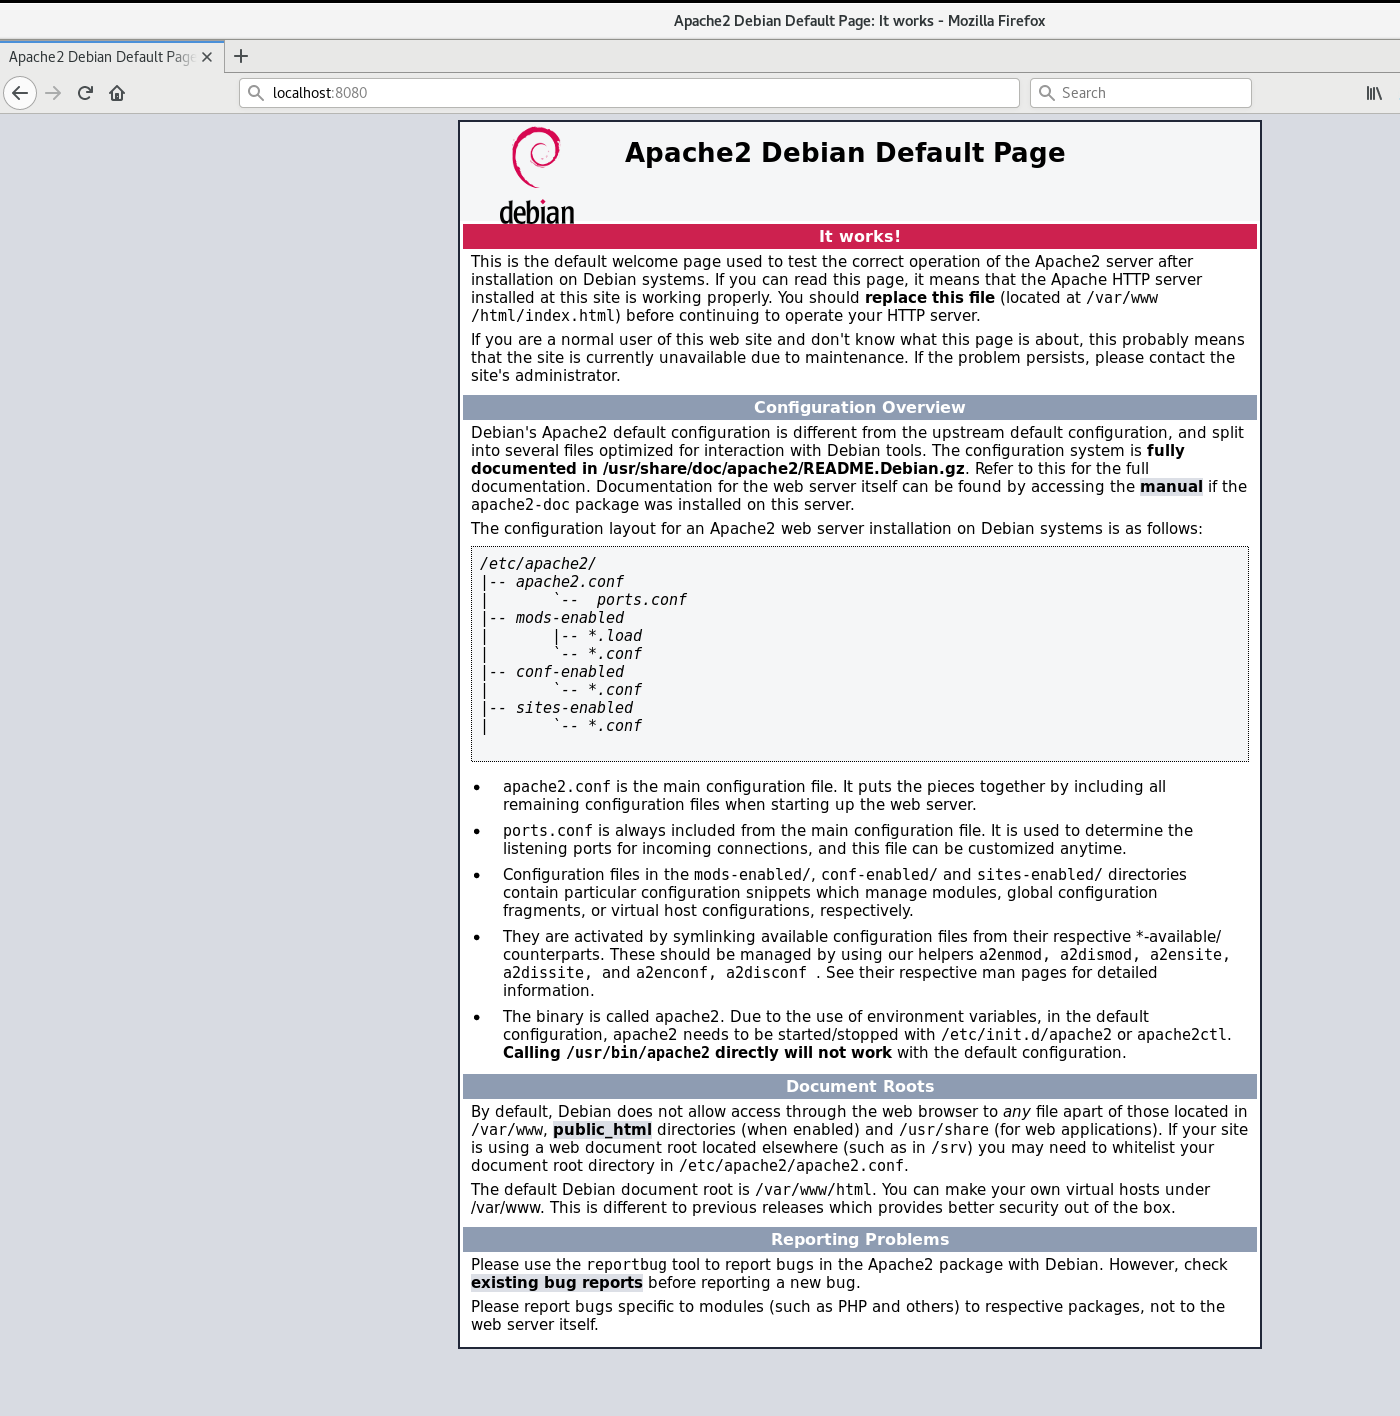
\includegraphics[scale=0.25]{resources/02.png}
  \caption{Page d'acceuil "It Works" d'Apache}
\end{figure}
Nous pouvons ajouter une page d'infos php dans la racine du serveur apache (par défaut /var/www/).\\
Puis nous activons les modules apache nécessaires avec \texttt{aen2mod}. \\
\begin{tcolorbox}
  \begin{verbatim}
    $ echo -e "<?php\nphpinfo();\n?>" > /var/www/html/info.php
    $ a2enmod mpm_prefork && a2enmod php7.0
  \end{verbatim}
\end{tcolorbox}
Nous pouvons voir la page d'infos sur l'adresse \texttt{localhost:8080/info.php}
\begin{figure}[!htp]
  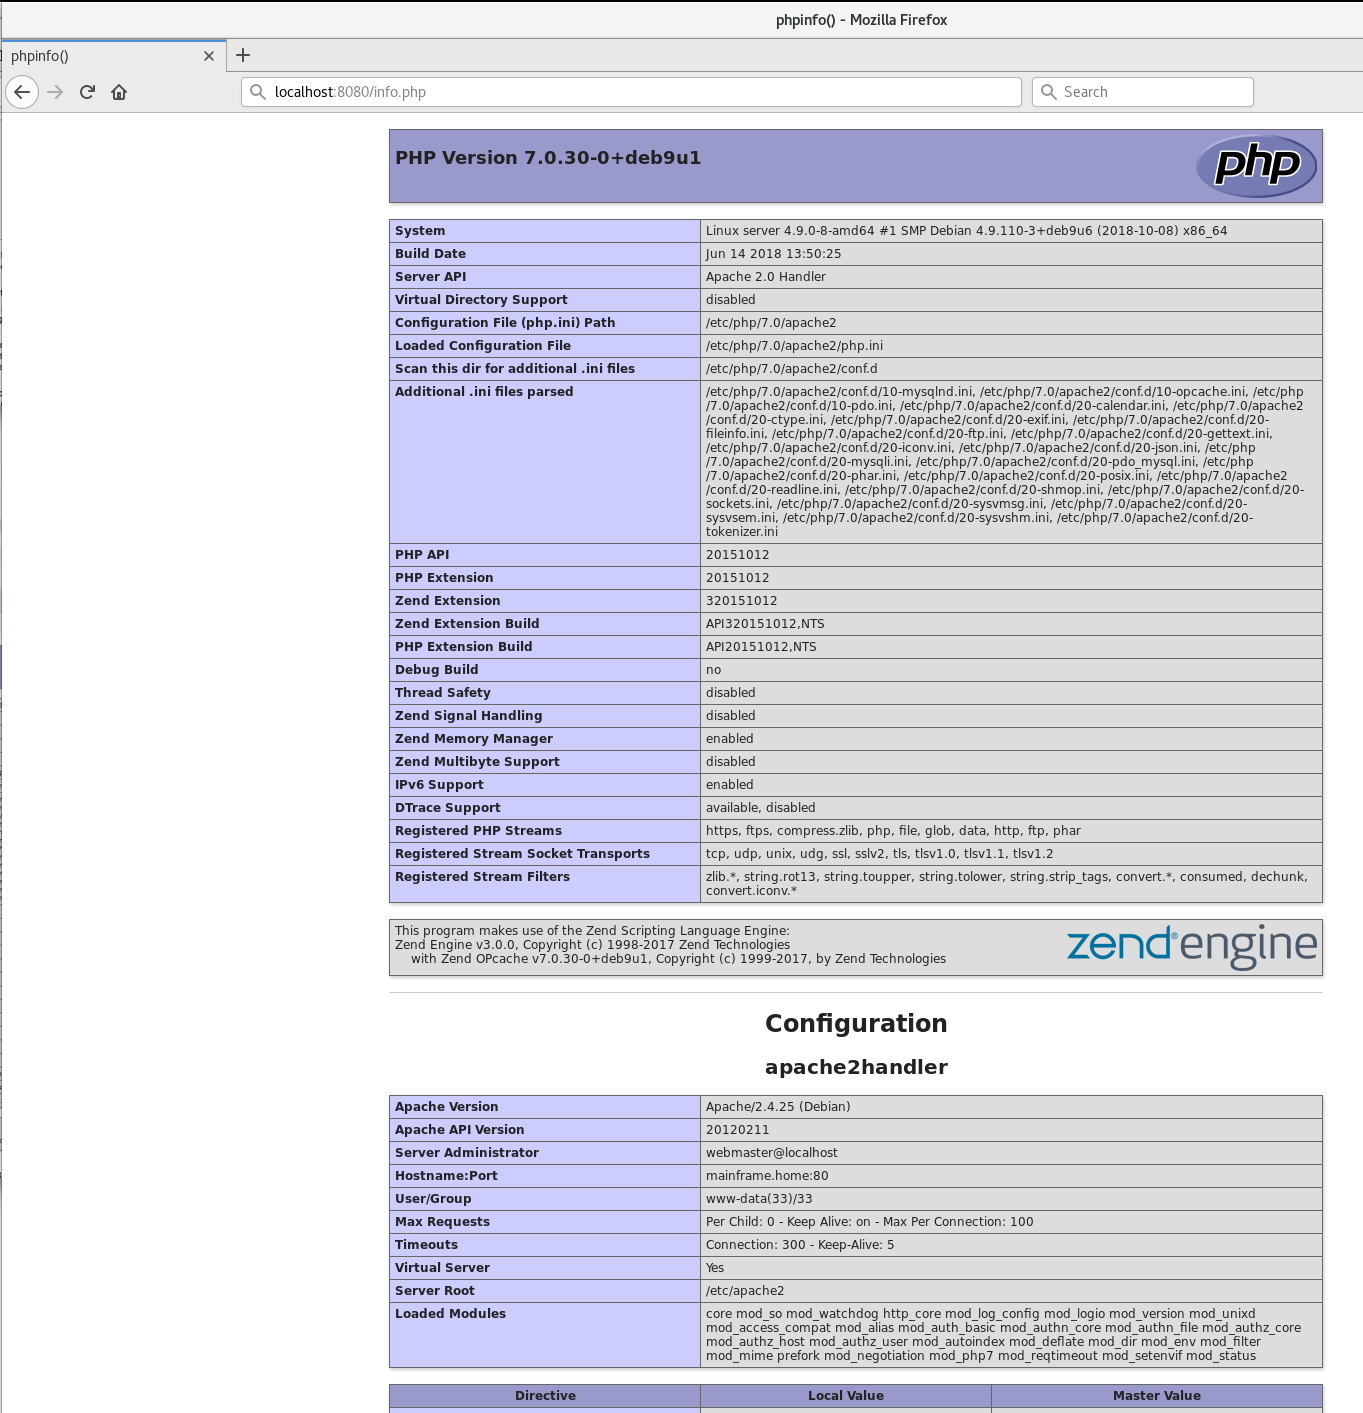
\includegraphics[scale=0.25]{resources/03.png}
  \caption{Page d'infos sur la machine générée par PHP}
\end{figure}

\subsection{Exercice 9}
Installation du package \texttt{mysql-server}
\subsection{Exercice 10}
Configuration de MySQL avec \texttt{mysql\_secure\_installation}
\subsection{Exercice 11}
Installation du package \texttt{phpmyAdmin} puis choisir les bonnes options.\\
Puis redémarrer le serveur apache et accèder à l'application web phpMyAdmin sur le lien : \\
\texttt{localhost:8080/phpmyadmin}

\subsection{Exercice 12}
\subsubsection{MySQL}
Nous allons configurer la base de données mySQL (maintenant mariadb)
\begin{tcolorbox}
  \begin{verbatim}
    $ mariadb
    #nouveau utilisateur wpuser
    $ CREATE USER 'wpuser'@'localhost' IDENTIFIED BY 'wpuser';`
    #nouvelle db wpdb
    $ CREATE DATABASE wpdb DEFAULT CHARACTER SET
    'utf8' COLLATE 'utf8_unicode_ci';
    #accorder toutes les permissions sur wpdb à wpuser
    $ GRANT ALL ON `wpdb`.* TO `wpuser`@`localhost`;
    #actualiser les tables de permissions
    $ FLUSH PRIVILEGES;
    $ exit
  \end{verbatim}
\end{tcolorbox}
\subsubsection{WordPress}
Installation du package \texttt{wordpress}.
Modification des fichiers \texttt{000-default.conf} et \texttt{default-ssl.conf} qui permettent
de configurer les liens mis à disposition des clients par apache.\\
Nous rajoutons les lignes suivantes sous la directive \texttt{DocumentRoot /var/www/html} :
\begin{tcolorbox}
  \begin{verbatim}
  Alias /istyblog /usr/share/wordpress
  <Directory /usr/share/wordpress>
      Options FollowSymLinks
      AllowOverride Limit Options FileInfo
      DirectoryIndex index.php
      Require all granted
  </Directory>
  <Directory /usr/share/wordpress/wp-content>
      Options FollowSymLinks
      Require all granted
  </Directory>
  ---------------------------------------------------
  Recharger apache avec :
  $ systemctl reload apache2
  \end{verbatim}
\end{tcolorbox}
Configurer le site pour utiliser MySQL/MariaDB dans /etc/wordpress/config-localhost.php :
\begin{tcolorbox}
  \begin{verbatim}
  <?php
  define('DB_NAME', 'wpdb');
  define('DB_USER', 'wpuser');
  define('DB_PASSWORD', 'wpuser');
  define('DB_HOST', 'localhost');
  define('WP_CONTENT_DIR', '/usr/share/wordpress/wp-content');
  ?>
  \end{verbatim}
\end{tcolorbox}

\subsection{Exercice 13}
Il faudra rajouter une nouvelle règle pour rediriger le port 443 afin d'utiliser https .\\
Puis utiliser iptables comme avant, et activer le module ssl d'apache.
\begin{tcolorbox}
  \begin{verbatim}
  $ Adding rule  Rule 4  TCP  127.0.0.1  9443  0.0.0.0  443
  $ iptables -t nat -A PREROUTING -p tcp -i enp0s3 --dport 443
    -j DNAT --to-destination 192.168.0.11:443
  $ iptables-save > /etc/iptables/rules.v4
  $ a2ensite default-ssl
  $ a2enmod ssl
  $ systemctl restart apache2
  \end{verbatim}
\end{tcolorbox}
Nous pouvons accèder à notre site d'acceuil avec https via : \texttt{https://localhost:9443}.
Cependant notre site wordpress ne fonctionne pas, il faudra changer les champs WordPress Address
et Site Address en modifiant le port et en mettant \textit{https} au lieu de \textit{http} dans
Settings > General.\\
Nous remarquons que l'émetteur du certificat SSL n'est pas reconnu.\\

\subsection{Exercice 14}
Si un attaquant parvient à obtenir la clé privée de notre paire, il peut voler l'identité du site,
puis voler les données des visiteurs du sites, et autres informations.

\begin{tcolorbox}
  \begin{verbatim}
  \end{verbatim}
\end{tcolorbox}
\end{document}
